% 用于记录一些常见的机器学习, 深度学习的概念

\subsection{L1/2 regularization}
$L1, L2$ 正则即在优化函数的基础上加上参数的 $L1, L2$ 范数, 即 $L1(\boldsymbol{w}) = \sum_{i=1}^{n} |w_i|$, $L2(\boldsymbol{w}) = \sum_{i=1}^{n} w^2$. 这里从梯度的角度阐述一下二者的区别, 这里仅求范数对参数的导数, 并省略了一些常数. 

$L1$: 
$$
\begin{aligned}
	\frac{\partial L1}{\partial w_i} &=  \text{sign}(w_i) \\
	w_i &= w_i - \eta\ \text{sign}(w_i)	
\end{aligned}
$$

$L2$: 

$$
\begin{aligned}
	\frac{\partial L2}{\partial w_i} &=  w_i \\
	w_i &= w_i - \eta\ w_i
\end{aligned}
$$
通过上述参数更新方式的对比, 可以很明显地看到 $L1$ 约束更新参数时只与参数地符号有关, 因此, 当 $w_i \in [1, +\inf)$ 时, $L2$ 能够更快地减小参数, 而当 $w_i \in (0, 1)$ 时, $L1$ 能更快地减小参数, 更容易使参数接近 0, 即小于 1 地参数有更大概率接近 0. 

当然, 除了从梯度的角度解释, 还可以从优化的角度和概率的角度. $L1$ 假设参数服从 Laplace 分布, 而 $L2$ 假设参数服从 Gaussian 分布, 从这两个分布 (标准的 Laplace 分布和标准的 Gaussian 分布) 的形状也可以看出 $L1$ 正则化下的参数有更大的概率接近或等于 0. 

\subsubsection{L1/2 的先验分布}
机器学习通常是在给定观察到的数据后对模型的参数进行估计, 相当于求后验概率: 
$$
MAP = \log P(y | X, w) P(w) = \log P(y | X, w) + \log P(w)
$$
即后验概率为似然函数加上参数的先验. 若假设 $w$ 的先验服从 0 均值的正态分布, 则: 
$$
\log P(w) = \log \prod_{j} P(w_j) = \log \prod_{j} \frac{1}{\sqrt{2 \pi } \sigma} e ^ {-\frac{w_j^2}{2 \sigma^2}} =-\frac{1}{2 \sigma^2} \sum_j w_j^2 + C
$$
可以看到, 在高斯分布下 $\log P(w)$ 的效果等价于在代价函数中增加了 L2 正则项. 若 $w$ 服从均值为 0, 参数为 $a$ 的拉普拉斯分布, 则: 
$$
\log P(w) = \log \prod_{j} P(w_j) = \log \prod_{j} \frac{1}{\sqrt{2 a} \sigma} e^{-\frac{|w_j|}{a}} = -\frac{1}{2a} \sum_j |w_j| + C
$$
可以看到, 在拉普拉斯分布下 $\log P(w)$ 等价于在代价函数中增加了 L1 正则项. 

\begin{flushright}
	
\end{flushright}参考: \href{https://www.zhihu.com/question/37096933/answer/475278057}{l1 相比于 l2 为什么容易获得稀疏解? - ser jamie的回答}. 


\subsection{判别模型、生成模型}
\begin{itemize}
	\item 判别模型: 直接对判别函数或者条件概率分布函数进行建模, 不考虑样本的产生模型, 直接研究预测模型
	\item 生成模型: 学习联合概率密度$P(Y, X)$, 然后求出条件概率分布$P(Y|X) = \frac{P(X, Y)}{P(X)}$, 不仅要求出联合分布, 还要求出训练数据的分布$P(X)$ ({\color{red}{不一定要计算$p(X)$, 因为对于同一个样本, 计算它属于不同分类时, 其$p(X)$是一样的, 对判别没有帮助}}) . 生成模型表示了输入$X$产生输出$Y$的生成关系
\end{itemize}

对于生成式模型, 可以这样理解: \\
$p(x | y) = p(y)p(x | y)$表示的是, 从$p(y)$中采样一个$y$, 然后根据$p(x|y)$采样一个$x$. 生成式模型希望找到那个能够使$p(x, y)$最大的$y$. 1


生成模型从统计的角度表示数据的分布情况. 判别模型不能反映训练数据本身的特性, 但它不断寻找不同类别之间的最优分类面. 

也可以从 \textbf{决策函数$Y=f(X)$或条件概率分布$P(Y|X)$} 的角度来看待判别模型和生成模型: 
从数据中学习一个分类器时, 希望通过给定的输入$X$输出相应的$Y$. 这个模型的一般形式为: 
\begin{itemize}
	\item 决策函数$Y=f(X)$: 输入一个$X$就输出一个$Y$, 可以将$Y$于阈值比较得到$X$的类别
	\item 条件概率分布$P(Y|X)$: 输入一个$X$, 输出$X$属于各个类的概率, 如$P(c_1 | X), P(c_2 | X)$. 取其中最大的作为$X$的类别
\end{itemize}
实际上$P(Y|X)$是隐含了或者说可以转化为决策函数形式$Y=f(X)$的. 例如, 将条件概率分布改写为$Y = \frac{P(c_1 | X)}{P(c_2 | X) }$. 

参考资料: \href{https://blog.csdn.net/fishmemory/article/details/51711114}{判别模型(Discriminative model)和生成模型(Generative model)}、\href{https://developers.google.cn/machine-learning/gan/generative?hl=zh-cn}{Background: What is a Generative Model?}. 

\subsection{熵、相对熵、交叉熵、互信息} 
\textbf{\checkmark 2020-10-08}\\
这些概念来自信息论\cite{6773024}. 简单来说, 熵指的是不确定性或者信息量, 熵越大不确定越大. 相对熵也叫KL(Kullback-Leibler divergence)散度, 用来比较两个概率分布之间的差异. 不论是熵、相对熵、交叉熵, 都可以看作针对某个 (或多个) 随机变量, 对该随机变量的概率分布的一个某种熵 (熵、相对熵、交叉熵) 的计算. 接下来就从数学上来对其进行描述. 

\textbf{熵}: 先介绍自信息的概念. 对于某个随机变量$X$, 当$X$取值为$x_0$时的自信息为$I(x_0) = -log\ p(x_0)$, 即事件$x_0$发生时所带来的信息量, 如果一个事件发生的概率越大, 则其带来的信息量越小. 熵是自信息的均值. 即$X$取任一值时所能带来的期望信息量, 故$X$的信息熵$H(X) = -E_{x\sim p}I(x)$ (其中p是$X$所服从的分布) , 即$H(X) = -\sum_{x \in X}log\ p(x)$. \textbf{因为随机变量$X$会服从某个分布, 假设是$p$, 则$H(X)$也可以看作是概率分布$p$的信息量的期望. }

\textbf{相对熵}: 也称作KL散度. KL是在信息熵的基础上定义的, 用来衡量两个分布的差异, 其实由上述熵的含义可知, 其实KL也可以看作是随机变量$X$, 其可能服从的两个分布之间的差异. 假设可能服从的两个分布分别是$p, q$, 则以$q$去接近$p$时的KL散度表示为: $D_{KL}(p||q) = \sum_{x \in X} p(x) log\ \frac{p(x)}{q(x)} = E_{x\sim p} log\ \frac{p(x)}{q(x)}$. 经过化简可得$D_{KL} = -H(p) + \sum_{x \in X}p(x)log\ q(x)$. 

\textbf{交叉熵}: \label{ce}cross-entropy, 与KL散度相似, 也是用来衡量随机变量$X$可能服从的两个分布$p, q$之间的差异的. 其数学上的定义为: $Cross-Entropy(p, q) = -E_{x\sim p} log\ q(x) = - \sum_{x \in X}p(x)log\ q(x)$. 很显然, 交叉熵比KL散度多了一个$H(p)$, 即$Cross-Entropy(p, q) = D_{kL}(p || q) + H(p)$. 

机器学习中常使用交叉熵, 既然KL散度和交叉熵都可以达到相同的目的, 那为什么不使用KL散度呢?在机器学习中, 上述的分布$q$常作为数据的真实分布, 而$q$作为数据的预测分布, 此时$H(P)$则可以视作一个常数 (因为给定数据后, 其真实分布是确定的) , 在优化模型的参数时, $H(P)$并不会对参数的优化做出贡献 (不会影响优化过程) , 故使用交叉熵即可. 

\subsection{关于交叉熵损失函数的一点理解}
交叉熵损失函数可以从多个角度进行理解. 从概率论的角度, 在极大似然概率估计中, 希望参数能够使得已有样本出现的概率最大. 

\paragraph{二分类}
在分类任务中, 由于不同样本是有标签的, 样本出现的概率应该与标签对应, 例如p表示1样本出现的概率, 则1-p表示0样本出现的概率, 那么对于1样本极大化的应该是p, 对于0样本极大化的应该是1-p. 

样本的极大化后的概率取对数后为相加的形式. 则对于一个样本, 其极大化的表示可以写成$log p$  (1样本) , 或者$log(1-p)$ ( 0样本) . 如果用一个统一的式子表示的话, 可以写成$y log p + (1-y) log(1-p)$, 其中y取0或1. 

通常是对损失函数最小化, 所以可以在极大化的表示前加个符号就变成了交叉熵损失函数: $- y log p - (1-y) log(1-p)$. 将一个batch里的样本的损失累加起来就是常见的形式了. 并且, 在用模型计算p时, p通常通过一个函数来表示$f(x)$, x即为输入的样本, $f(x)$可以是各种机器学习模型, 如逻辑回归、神经网络等. 


\paragraph{多分类}
对于一个$C$个类别的多分类任务, 用$p_i$表示样本$x$被预测为第$i$类的概率, $x$的真实类被为$c$, 也可以用一个one-hot向量$y = [y_1, y_2, ..., y_C],\ y_i = 1\ if\ i = c\ else\ y = 0$表示$x$的真实类别. 那么$x$的损失即可表示为$loss_x = \sum_{i=1}^C y_i\ \log p_i$. 显然, $loss_x = \log p_c$. 通常, 如果$\{p_i\}_{i=1}^C$是未归一化的, 那么实践中, $loss_x = \log \frac{e^{p_c}}{\sum_{i=1}^C e^{p_i}}$

除了从极大似然的角度来理解交叉熵损失函数, 当然也可以直接从交叉熵\ref{ce}的角度来理解. 

\subsection{方差与偏差}
\paragraph{偏差 (Bias) }通常是指: 对于一种模型, 它的平均 (训练多次也就得到了多个模型实例) 预测结果与真实值之间的差距. 偏差度量的是学习到的函数与真实函数的差距的期望, 即$E[\hat{f} - f]$. 

\paragraph{方差 (Variance) }选用一种模型 (如KNN, SVM, NN等) , 使用不同的数据集可以得到该种模型的多个实例 (即训练好参数的模型) . \textbf{这些模型}对于同一个输入给出的预测值的方差, 即$E[(\hat{f} - E[\hat{f}])^2]$. 方差是受所使用的训练集影响的, 我们使用不同分布的数据集训练出来的模型会导致学出来的模型参数变化, 这反映出来的就是针对同样的输入会产生不一样的预测值, 这些预测值的方差就反映了模型的方差. 

在模型很复杂的时候, 在训练集上学习的模型能够准确地预测, 产生较小的偏差, 但是更容易产生大方差, 因为模型有更多的参数, 能够“死记硬背”记下输入与输出的映射关系, 这个时候模型可能记住了一些没用的东西甚至是噪声, 而模型是没有见过测试集的, 稍微有些不同的数据点的输出可能会有较大的差别, 从而产生大的偏差.  --- \textbf{过拟合}

当模型较简单的时候, 可能无法充分地利用训练集, 在测试集上会产生较大的偏差, 但是因为模型参数少, 模型关注地特征较少, 光从这些特征来看的话, 测试集中的数据与训练集中的数据会有更高的相似性, 因此就算不同的数据输入, 但是由于某些特征被忽略后数据反而是相似的, 所以模型给出的输出是类似的, 因而方差小. --- \textbf{欠拟合}

参考: \href{http://scott.fortmann-roe.com/docs/BiasVariance.html}{Understanding the Bias-Variance Tradeoff}, \href{http://www.r2d3.us/visual-intro-to-machine-learning-part-2/}{Model Tuning and
	the Bias-Variance Tradeoff} (可视化解释, 墙裂推荐) , \href{https://www.cnblogs.com/makefile/p/bias-var.html}{偏差方差分解} (分解过程的详细推导) . 


\textbf{注意: }\textbf{一种模型相当于一个函数空间}, 当我们选择一种模型进行训练, 得到了该种模型的各个参数, 就相当于得到了一个实例化的模型. 模型种类相当于类, 训练好的模型相当于对象. 喂数据训练模型时相当于在某个特定的函数空间中找到一个合适的函数 --- 即我们要的模型. 有时候训练后的模型效果不好, 可能不是这种模型不行, 可能是没有在这个函数空间中找到合适的函数. 

\subsection{交叉验证}
在训练模型的时候, 通过会把数据集划分为训练集和测试集, 测试集的作用用于学习模型参数, 测试集是为了检验模型在未见过的数据上的效果. 但是只将数据集划分为测试集和训练集有以下问题: 
\begin{itemize}
	\item 最终模型与参数的选取将极大程度依赖于你对训练集和测试集的划分方法. 不同的划分情况, 学习出来的参数是不一样的; 固定模型参数, 模型在不同划分上的表现也是不一样的. 这种情况使得我们无法准确对模型的能力进行评估, 不利于我们选择最优的模型 (指何种模型) 以及最优的模型参数 (一般是指超参数, 而不是模型学习到的参数) ; 
	\item 该方法只用了部分数据进行模型的训练, 无法充分利用已有的数据. 测试的效果只是针对某个划分, 并不是针对整个数据集, 不够有说服力; 
\end{itemize}
为了解决以上为题, 即1) 选择最好的模型与参数; 2) 充分利用数据, 使模型的测试结果有说服力, 就有了交叉验证 (Cross Validation) . 常见的交叉验证方法: 
\begin{itemize}
	\item LOOCV (Leave-one-out cross-validation) , 即留一验证. 对于有N个样本的数据集, 重复N次, 每次选择其中一个作为测试集, 其他的作为训练集, 这样就得到了N个$(train_i, test_i), i = 1, ..., N$训练集、测试集对儿. 分别用这N个训练集-测试集对儿来训练模型, 这样就可以学习到N个模型. 每个模型都可以得到一个测试得分, 进行平均后就作为这类模型在这个数据集上的测试分数
	
	\item K-fold CV, 即K折交叉验证. 与LOOCV类似, 但是对数据集的划分不同, 是把数据集划分为K份, 每次取其中一份作为测试其, 其余作为训练集, 这样就可以得到K个测试得分, 进行平均后作为最终的测试分数
\end{itemize}
\textbf{注意: 给定模型种类和一组超参数, 这样就确定了一个模型, 但是模型的参数需要通过数据来学习 (如Fig.\ref{fig:model}所示) , 比如线性回归中的权重, 上述的N个或K个模型是针对某个模型种类和一组超参数组合而言, K或N个不同的训练集学习到的K或N个模型, 但它们的超参数都是一样的}, 具体过程就是: \tbc{red}{确定模型类别 ==> 确定超参数 ==> 喂数据进行学习 (喂K次不同的数据)  ==> 得到K个模型 (但是超参数都一样)  ==> 计算平均得分 ==> 得到这种模型在这种超参数下的得分}, 这也就是CV可以用于选择模型 (\textbf{选择模型最优的超参数}) 的原因. 

\begin{figure}[h]
	\centering
	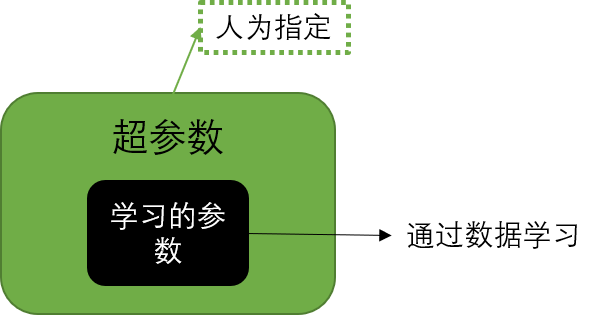
\includegraphics[width=.5\textwidth]{pics/model.png}
	\label{fig:model}
	\caption{模型的超参数与学习参数}
\end{figure}

一些值得注意的问题: 
\begin{itemize}
	\item LOOCV计算成本太高而且不同训练集之间的重合度太高
	\item K的选取. K太大, 投入的训练集也大, 得到的模型可能会有较小的偏差, 但是由于训练集之间的重叠度较高, 会存在较高的方差
\end{itemize}

\subsection{归一化 vs 标准化 定量的分析}
参考: \href{https://mp.weixin.qq.com/s/lO3Li7dWAvtzefVA_M0dJg}{https://mp.weixin.qq.com/s/lO3Li7dWAvtzefVA\_M0dJg}\\
\textbf{归一化: }将值变换到$[0, 1]$或者$[-1, 1]$之间, 使得不同类型的特征之间有了可比性, 对利用了样本之间距离的算法很重要. \textbf{标准化: }改变数据的统计特征, 如将均值和方差变为0和1. 在现实中, 一个变量极有可能是服从正态分布的. 


一些重要的结论: 
\begin{itemize}
	\item 对于不同的算法, 可能不同的缩放方法有不同的效果, 例如Tree-based模型对特征的尺度是不敏感的, 而一些依赖样本之间的距离的方法则对尺度很敏感, 如KNN、LR等; 
	
	\item 归一化容易受到异常值的影响, 可能会将数据点挤压到一起; 
\end{itemize}

二者的使用场景:
\begin{itemize}
	\item 标准化. 更好地保留了样本间的间距,因此在一些依赖距离度量的算法中,例如 分类, 聚类中最好使用规范化;
	
	\item 归一化. 如果数据不太符合正态分布, 或者对数据的范围有要求可以使用归一化;
\end{itemize}

\subsection{数据探索}
\paragraph{What?}数据探索是机器学习任务中的一个过程, 通过数据探索, 我们应该能够对数据有一个深入的认识. 很多人认为数据探索只是任务开始之前的一个步骤, 其实数据探索应该\textbf{贯穿整个任务的生命周期}. 在任务开始前, 对数据有个整体的把握, 知道数据的形式、数据量、数据的异常、缺失值、冗余等; 在完成任务的过程中, 发现当前使用的特征的特点, 特征的价值、关联等; 完成任务后, 分析特征的重要性、误差, 以及可能的优化方向. \textbf{数据探索, 是我们选用何种算法的依据, 以及算法模型中使用哪些特征. }

\paragraph{How?}
\subparagraph{数据初探}认识数据, 掌握原始数据的基本情况, 通过这一步, 我们要做到: 
\begin{itemize}
	\item 数据集的基本情况: 数据集有多大、数据的形式、数据的类型
	\item 重复值、缺失值、异常值: 去除重复值, 缺失值的处理, 缺失是否严重、是否有特殊含义, 发现异常值并处理
	\item 特征之间的冗余性: 是否有特征重复表达了
	\item 是否存在时间信息: 引入时间后, 处理会更复杂, 通常要进行相关性、趋势、周期和异常点的分析, 以及潜在的数据穿越问题
	\item 标签分布: 分类问题中类别分布是否均衡、回归问题中是否有异常值、值的分布情况、\textbf{是否需要进行目标转换}
	\item 训练集与测试集的分布: 训练集与测试集中标签的分布是否一致、两个数据集是否同分布
	\item 单变量/多变量分析: 特征的分布、特征之间的关系、特征与目标变量的关系
\end{itemize}
了解数据长什么样后, 我们才能知道\textbf{该选用哪个算法模型}、\textbf{该如何处理数据}、对数据进转换. 

\subparagraph{变量分析}分析特征的特点、特征之间的关联, 冗余性等. 主要可以分成: 
\begin{itemize}
	\item 单变量分析: 按照变量的取值, 可以将变量分为连续性和离散型. 连续性一般为数值, 离散型则比较多了, 如类别型、字符串、日期等. 单变量分析分析标签、特征的分布, 特征与目标的相关性等. 挖掘特征图用目标的关联, 可以帮助去除无效的特征, \textbf{找到有效的特征组合 (特征交叉) }, 如强相关加弱相关、强相关加强相关等
	
	\item 多变量分析: 分析特征变量之间的关系. 帮助我们发现哪些特征是冗余的, 进行特征组合, 发掘更高阶的特征
\end{itemize}

\subparagraph{模型分析}任务完成或者模型训练完后, 一般还需要对算法进行调整, 这时候就需要通过分析正在使用的模型有哪些缺点, 主要的方式有: 
\begin{itemize}
	\item 学习曲线: 发现是否存在过/欠拟合的问题
	\item 特征重要性分析: 通常在得到模型后, 我们可以获得特征的重要性, 分析特征的重要性是否符合实际情况、或者发现不符合直觉的深层现象、帮助我们选择特征
	\item 误差分析: 通过模型预测结果发现问题. 回归中看预测结果的分布, 分类中看混淆矩阵等. 借此来发现对于哪些样本表现不佳, 找到模型的弱点, 或者\textbf{为什么在这些样本上不佳的原因, 有时我们需要赋予这些 hard 样本更高的权重}
\end{itemize}





\subsection{Inductive Bias}
归纳偏置, 使用某个算法解决问题时所基于的假设, 类似于贝叶斯中的先验 (prior) , 与先验不同, 归纳偏置在学习过程中不会被更新, 而先验会不断被更新. 机器学习中常见的归纳偏置: 奥卡姆剃刀、CNN中的局部性、KNN中假设相似样本在特征空间中也是相邻的、SVM假设好的分类器应该是类别边界距离最大的等. 

\subsection{Covariate Shift}
协变量偏移, 指机器学习中训练集和测试集样本分布不一致的现象. 机器学习中通常假设训练和测试数据的分布是一致的, 在训练集学习的参数能否在测试数据上也有很好的表现呢?当训练集和测试集的分布不是那么相似时, covariate shift就出现了. 这里的数据分布不一致举个例子: 训练一个健康预测器, 训练集大多是 60 岁以下的, 但是测试集却大部分来自老年人. 

\subsubsection{怎么发现 Covariate Shift?}
做机器学习任务, 检验训练集和测试集的分布是很重要的, 其实一直不太了解如何验证两个数据集的分布是否一致. 验证是否发生了 Covariate Shift 其实也可以看作验证训练集和测试集的分布是否一致. 既然时验证分布是否一致, 那么就可以看成是一个分类任务, 训练一个分类器来判断一个样本是来自训练集和测试集. 具体做法: 从训练集和测试集中随机挑选等量的样本, 生成一个新的数据集, 给这个数据集中的每个样本增加一标签, 标识其来自训练集还是测试集, 之后就用这个新数据集进行训练, 训练完后计算模型的性能, 如果性能不错, 则说明出现了偏移. 

\subsubsection{怎么解决?}
怎么解决呢?
\begin{itemize}
	\item 训练集和测试集的分布不一致导致模型的参数泛化性能不佳, 可能是测试集中地某些样本在训练集中被“轻视”或“过度重视”了, 因此可以通过附加一个权重来解决该问题. 可参考: \href{https://blog.csdn.net/mao_xiao_feng/article/details/54317852}{covariate shift现象的解释}; 
	\item 丢弃那些导致偏移的且不重要的特征, 参考: \href{https://zhuanlan.zhihu.com/p/205183444}{Covariate Shift}. 
\end{itemize}

\subsection{机器学习中常用的算法指标及其应用场景}

% Please add the following required packages to your document preamble:
% \usepackage{multirow}
% \usepackage[table,xcdraw]{xcolor}
% If you use beamer only pass "xcolor=table" option, i.e. \documentclass[xcolor=table]{beamer}
\paragraph{Accuracy, Recall, Precision, F-score}

$ACC = \frac{TP + TN}{TP+FN+TN+FP}\quad R = \frac{TP}{TP+FN}\quad P = \frac{TP}{TP+FP}\quad F(\beta) = (1 + \beta^2)\frac{P \cdot R}{\beta^2 P + R}$. 混淆矩阵 (Confusion Matrix) 见表.\ref{tab:confusion_mat}. F-score是对R, P的一个综合评价, $\beta$度量了R 相对于 P的重要性, 可以理解为$\beta = \frac{importance(R) }{importance(P)}$, 则表示$\beta$越大, 我们越看重R. 

\begin{table}[h]
	\centering
	\caption{二分类混淆矩阵}
	\label{tab:confusion_mat}
	\begin{tabular}{|c|l|l|}
		\hline
		\multicolumn{1}{|l|}{}                          & \multicolumn{2}{c|}{Actual class (observation)}                                                                                   \\ \hline
		& tp (true positive) Correct result                          & fp (false positive) Unexpected result                                \\ \cline{2-3} 
		\multirow{-2}{*}{Predicted class (expectation)} & \cellcolor[HTML]{68CBD0}fn (false negative) Missing result & \cellcolor[HTML]{68CBD0}tn (true negative) Correct absence of result \\ \hline
	\end{tabular}
\end{table}

\paragraph*{关于$Precision$, $Recall$的选择?}这几个指标在很多任务中都有应用, , 但是不同的指标侧重于不同的方面, 比如P、R都有不同的侧重, 但看一个指标是比较片面的, 并不能反映出模型真实的效果. 有可能P很高, 但是R很低, 而在一些场景下R是很重要的. 

比如在金融风控等领域, 我们希望算法能够尽量识别出所有有可能有风险的用户, 这时候就侧重于 Recall, 即希望算法把所有的正样本 (通常有危险的, 需要被找出来的被标记为正样本) 都筛选出来, 即使将所有样本都标为正 (即 Recall=1) . 因为这种情况下, 可能漏掉一个正样本带来的代价是极大的, 通常筛选完之后还需要交给人工进行判断. 类似的场景还有癌症检测, 将一个没有癌症的判断为癌症没有很大关系, 但是将一个有癌症的判断为没有癌症则是很严重的, 会出人命的!!!

又比如在垃圾邮件分类中, 我们可能更侧重于Precision. 我们希望算法在识别垃圾邮件时不要把正常邮件错分了, 这个时候希望Precision尽可能高, 即使将所有样本标为负也没关系 (TP=0时可认为Precision=1) , 或者说算法只把自己十分确信为垃圾邮件的标为正, 尽量降低FP, 即尽量不要把正常邮件视为垃圾邮件, 不然错过了offer那可咋整!!!

通常, 将需要识别出的类别, 或者简单的说坏的一类为正样本, 为什么呢?因为好的漏掉一般不会产生啥大的影响, 但是坏的跑了课就不行了!当然, 也需要不同场景下选择合适的指标!!!

我们是贪心的, 因此就有了一些综合的指标, 比如F-score. 
Precision是以被分类的所有样本为分母, Recall则是以原本所有的positives元素为分母. 二者之间并没有建立直接联系, 如果一个分类器, Precision很高但是Recall很低, 或者Recall很高但是Precision很低, 这两种分类器都是不好的, 都是我们不希望的. 所以我们采用F1-Score来建立Precision和Recall的联系. 

\textbf{在数学中, 调和平均数是永远小于等于算术均值平均数的, 当用于求两个数的平均数时, 如果直接用算术平均作为结果, 那么两数之间的差异将被大的值削平, 而调和平均数则不会极大削平这种大的差异, 得到的结果更倾向于小的值}. 

\paragraph{Micro-F1 \& Macro-F1}基本的F1使针对二分类任务而言的, 在多分类中中, Micro-F1和Macro-F1是两种求多类别F1均值的方式. 
\begin{itemize}
	\item Micro-F1: 分别计算每个类别的$TP, FN, FP$, 再求整体的$Recall$, $Precision$, 再以整体的$P, R$来求$F1$, 得到Micro-F1. 在计算公式中考虑到了每个类别的数量, 所以适用于数据分布不平衡的情况; 但同时因为考虑到数据的数量, 所以在数据极度不平衡的情况下, \textbf{数量较多的类 (即常见的类) 会较大的影响到F1的值}
	\item Macro-F1: 分别计算每个类别的F1, 再求平均, 得到Macro-F1. 没有考虑到数据的数量, 所以会平等的看待每一类 (因为每一类的precision和recall都在0-1之间) , \textbf{会相对受高$Precision$和高$Recall$类 (即稀有的类) 的影响较大}
\end{itemize}
$Micro-F1$公式如下所示: 
$$
\begin{aligned}
	 Recall_{m i} &=\frac{\sum_i TP_{i}}{\sum_i TP_{i} + \sum_i FN_{i}} \\
	Precision_{m i} &=\frac{\sum_i TP_{i}}{\sum_i TP_{i} + \sum_i FP_{i}} \\
	Micro-F1 &= \frac{ Recall_{m i} \times Precision_{m i}}{Recall_{m i}+ Precision_{m i}}
\end{aligned}
$$
$Macro-F1$如下所示: 
$$
Macro-F1 &=2 \frac{ \sum_i F1_i}{N}
$$


\paragraph{ROC、AUC}接收者操作特征曲线 (recevier operating characteristic curve) , 用于反映一个而分类器的灵敏度 (sensitivity) 和特异度 (specificity) 之间的关系. 
$$
\begin{aligned}
	Sensitivity &= \frac{TP}{TP + FN}\\
	Specificity &= \frac{TN}{TN + FP}
\end{aligned}
$$
其中Sensitivity也就是TPR (True Positive Rate) , 也就是Recall, Specificity是TNR (True Negtive Rate) . ROC的横坐标是$1 - Specificity$, 即FPR (False Positive Rate, 即\textbf{负样本中有多少被分成了正样本}) , 纵坐标是Sensitivity. 横坐标表示的是负样本中被预测为正样本的比例, 纵坐标表示的是正样本中被预测为正样本的比例. 

ROC如Fig.\ref{fig:roc}所示. 

\begin{figure}[h]
	\centering
	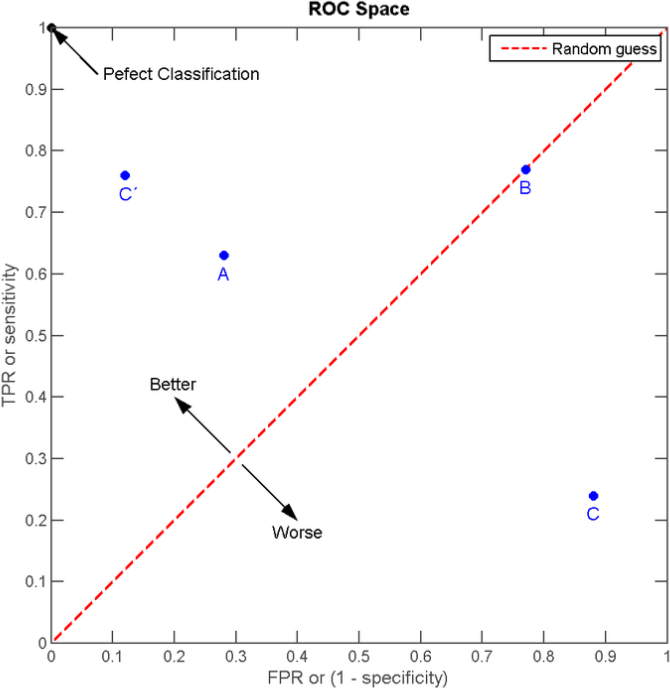
\includegraphics[width=.6\textwidth]{pics/roc.png}
	\caption{ROC}
	\label{fig:roc}
\end{figure}
ROC的绘制过程: 对于一个二分类问题, 使用一个分类器对样本集进行预测后, 可以得到每个样本属于正样本的概率, 此时我们还需要一个阈值来确定那些为正样本. 每选取一个阈值, 就可以得到一个 (TPR, FPR) 数值对. 当阈值从1到0不断减小时, 被确定为正样本的样本数不断增大, 其中TP和FP都会不断增大, 由于正负样本的数量是固定的 (即TPR, FPR的分母是固定的) , 则TPR和FPR都会不断增大. 那么, 
\begin{itemize}
	\item 当阈值为1时,  (几乎) 所有样本都为负样本, 则TPR约为0, 既然都为负样本那么FP也为0, 则FPR也为0
	\item 当阈值为0时, 所有样本都为正样本, 那么肯定所有的正样本都找出来了, 则TPR为1, 由于所有样本都预测为正样本, 那么肯定所有的负样本都预测为了正样本, 则FPR为1
\end{itemize}
因此, 在阈值从1到0的过程中,  (TPR, FPR) 不断增大, 从坐标 (0, 0) 到 (1, 1) , 如Fig.\ref{fig:threshold}所示, Fig.\ref{fig:threshold}上部分为负样本为正样本的概率的分布图 (即横坐标为正样本概率值, 纵坐标为对应的样本数量) , 下部分为正样本为正样本的概率的分布图, 可见, 当阈值为$B$时, 大部分正样本都被分为了正样本 (TP) , 小部分负样本被分为了正样本 (FP) . 由Fig.\ref{fig:roc-threshold}可见, 当阈值减小时,  (TPR, FPR) 的变化过程. 

\begin{figure}[h]
	\centering
	\subfigure[阈值变化与预测正负样本的分布]{
		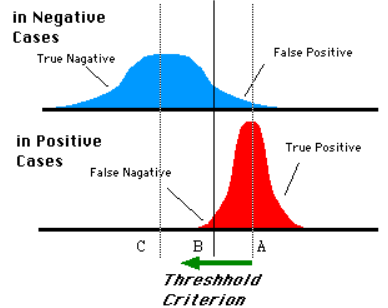
\includegraphics[width=7cm]{pics/threshold.png}
		\label{fig:threshold}
	}
	\quad
	\subfigure[阈值变化与ROC]{
		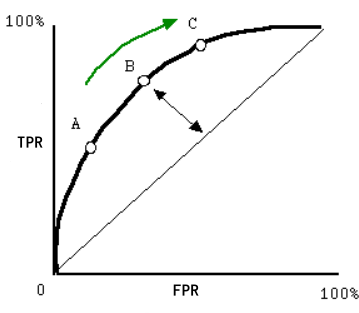
\includegraphics[width=7cm]{pics/roc-threshold.png}
		\label{fig:roc-threshold}
	}
	\caption{阈值变化}
	\label{fig:threshold-change}
\end{figure}
ROC是一个曲线, 那怎么作为一个指标呢? --- 取ROC与坐标轴围成的面积, 即\textbf{AUC (Area Under Curve) }. 由于ROC的绘制过程, 我们希望当阈值为接近0时, TPR尽量高, FPR尽量低 (其实不管阈值为何值, 都希望有这个效果) , 一个好的分类器的ROC的AUC应该尽量大. 

AUC的含义: 随机挑选一个正样本、一个负样本, 分类器分别给出一个分数, 正样本的分数大于负样本的分数的概率. \tbc{red}{强烈推荐}-相关证明: \href{http://vividfree.github.io/%E6%9C%BA%E5%99%A8%E5%AD%A6%E4%B9%A0/2015/11/20/understanding-ROC-and-AUC}{\tbc{red}{理解 ROC 和 AUC}} (以及 AUC 的简洁计算方式). 

\textbf{为什么要用ROC/AUC呢?}\newline
因为ROC曲线有个很好的特性: 当测试集中的正负样本的分布变化的时候, ROC曲线能够保持不变. 在实际的数据集中经常会出现类不平衡(class imbalance)现象, 即负样本比正样本多很多(或者相反), 而且测试数据中的正负样本的分布也可能随着时间变化. roc曲线不变原因: TPR和FPR是实际label内部的操作, 看混淆矩阵和tpr、fpr计算公式, 无论实际label比例怎么变化, tpr、fpr计算公式都是在实际为p或者n的内部计算的. AUC 关注的是样本间的排序效果. AUC 对正负样本比例的不敏感性: \href{https://blog.csdn.net/Leon_winter/article/details/104673047}{AUC: 直观理解AUC为何会对正负样本数分布不均匀情况鲁棒}. 

\textbf{如何使用ROC来选择模型?}\newline
当我们有多个分类器时, 给定一个数据集, 可以得到多条ROC曲线, 那么怎么来选择模型呢?一个很直观的想法是直接比较AUC. 但是在不同场景下, 我们要结合更看重的指标选择模型. 如Fig.\ref{fig:roc-cmp}所示, 当ROC不交叉时, 可以直接选择AUC高的, 当ROC交叉时则需要慎重考虑了. 当需要高的Sensitiviy时, 选择A, 需要高Specificity (即低FPR) 时选择B. 


\begin{figure}[h]
	\centering
	\subfigure[ROC不交叉]{
		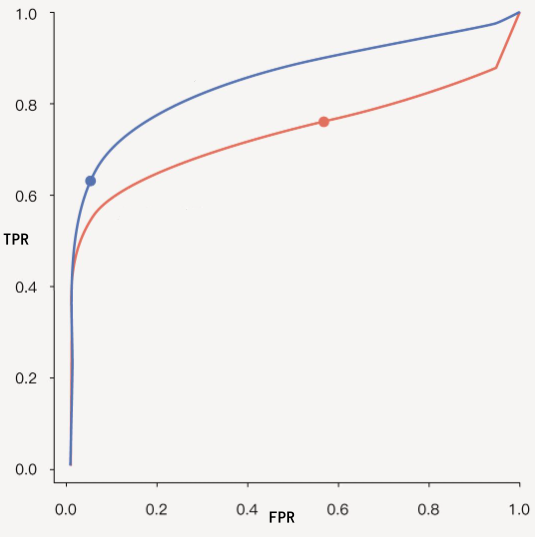
\includegraphics[width=7cm]{pics/roc1.png}
		\label{fig:roc1}
	}
	\quad
	\subfigure[ROC交叉]{
		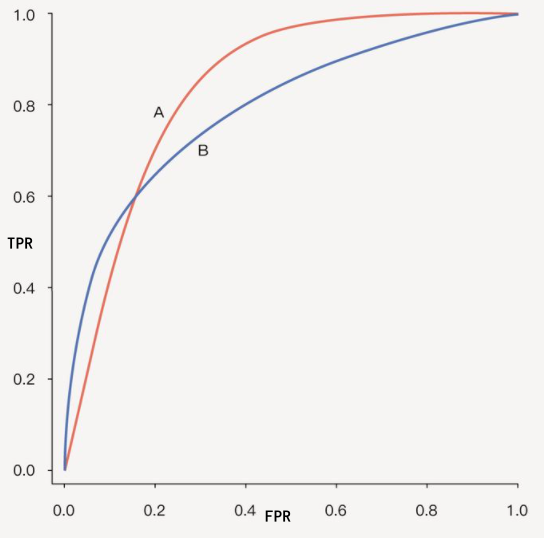
\includegraphics[width=7cm]{pics/roc2.png}
		\label{fig:roc2}
	}
	\caption{ROC比较}
	\label{fig:roc-cmp}
\end{figure}

参考资料: 
\begin{itemize}
	\item \href{https://blog.csdn.net/pipisorry/article/details/51788927}{分类模型评估之ROC-AUC曲线和PRC曲线}
	\item \href{https://zh.wikipedia.org/zh/ROC%E6%9B%B2%E7%BA%BF}{ROC曲线}
\end{itemize}


\paragraph{mIoU}
Mean Intersection over Union(MIoU, 均交并比), 为语义分割的标准度量. 其计算两个集合的交并比, 在\textbf{语义分割}的问题中, 这两个集合为真实值 (ground truth) 和预测值 (predicted segmentation) . 令$p_{ij}$表示实际类别为$i$, 预测类别为$j$的数量, 则
$$
mIoU = \frac{1}{C} \sum_{i=1}^{C} \frac{p_{ii}}{ \sum_{j=1}^{C} p_{ij} + \sum_{j=1} p_{ji} - p_{ii} }
$$
如下图Fig.\ref{fig:miou}所示: 
\begin{figure}[h]
	\centering
	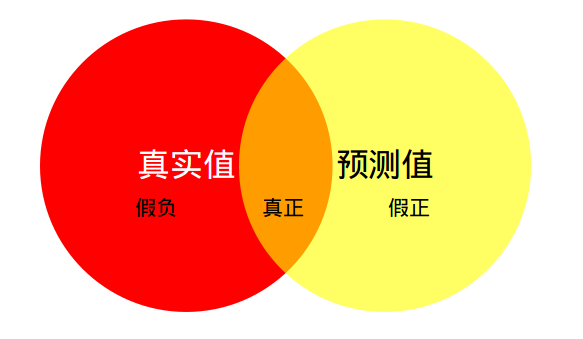
\includegraphics[width=.6\textwidth]{pics/miou.png}
	\caption{mIoU}
	\label{fig:miou}
\end{figure}
在\textbf{语义分割}中, 被分类的对象为每个像素, 真实标签为该像素所属的类别, 预测标签为预测的类别. 计算时, 可以先计算出混淆矩阵, 将对角线上的元素的值之和除以混淆矩阵中所有元素的和, 再除以类别数就是mIoU了. 注意, 在实际计算中, 要注意除零的情况. 

\paragraph{Dice}
有Dice系数和Dice loss之分. 
Dice系数是一种集合相似度度量函数, 通常用于计算两个样本的相似度, 取值范围在[0,1], 计算公式如下: 
$$
dice(x, y) = \frac{2|x \cap y|}{|x| + |y|}
$$
在\textbf{语义分割}中, $x, y$可以分别代表预测的分割结果、真实的分割, 分别以矩阵的形式表示. 那么, 计算模型的分割效果可以为: 
$$
dice(pred, ground) = \frac{2(pred \cdot ground).sum()}{pred.sum() + ground.sum()}
$$
其中, $\cdot$和\textit{.sum()}分别表示矩阵的逐元素乘积、逐元素求和. 
Dice loss则是: $1 - dice(pred, ground)$, Dice loss 首次在VNet中提出. 

在图像分割实践中, 可以用Dice loss或者交叉熵损失函数作为目标函数, 但是由于交叉损失函数的梯度形式更优, 更倾向于选择交叉熵损失函数. 
Dice Loss特点: 
\begin{itemize}
	\item 训练误差曲线非常混乱, 很难看出关于收敛的信息. 尽管可以检查在验证集上的误差来避开此问题
	\item Dice Loss比较\textbf{适用于样本极度不均的情况}, 一般的情况下, 使用 Dice Loss 会对反向传播造成不利的影响, 容易使训练变得不稳定
	\item Dice对mask的内部填充比较敏感
	
\end{itemize}
作为Dice loss的一个替代, 可以使用cross entropy loss. 原因: 
\begin{center}
	使用交叉熵做损失函数时, 在反向传播时, 计算得到的梯度的形式是类似于 (p-t) 的, 其中$p, t$分别是预测值和标签. 而dice loss, 如果将其写成$\frac{2pt}{p^2+t^2}$ 或 $\frac{2pt}{p+t}$的形式, 则在反向传播时, 梯度大概时这个样子的:  $\frac{2t(t^2-p^2)}{(p^2+t^2)^2}$ 或 $\frac{2t^2}{(p+t)^2}$. 这样的梯度有什么问题呢?当$p, t$都很小时, 梯度可能会变得很大, 这也是\textbf{dice loss在训练过程中不稳定的原因}了. 
\end{center}



\paragraph{Rand Error}
Rand Error是以Rand Index (兰德系数) 为基础的. Rand Index用于衡量两个数据簇之间的相似性. Rand Index的定义: 
对数据点集进行分类时, 用a表示实际为同一类, 预测时也为同一类的数据点对 (pair) 的数量, b表示实际为不同类, 预测时也为不同类的数据点pair的数量, 则
%\binom{n}{k}\qquad\mathrm{C}_n^k
$$
RI(Rand Index) = \frac{a + b}{\mathrm{C}_n^k}
$$
Rand Error定义为: 
$$
RE = 1 - RI
$$
RE可以用于衡量图像分割算法的效果. 可以参考: \href{http://www.otlet-institute.org/wikics/Clustering_Problems.html#toc-Subsection-4.1}{Rand Index计算}. 

\paragraph{Hausdorff 距离} 可以用于衡量两个点集之间的距离, 定义如下, 其中$\boldsymbol{X}, \boldsymbol{Y}, d(x, y)$表示两个点集和点之间的距离度量函数: 
$$
d_{H}(X, Y) = \max (d_{X Y}, d_{Y x}) = \max \left\{\underset{x \in X}{\max } \min _{y \in Y}d(x, y),\quad \max _{y \in Y} \min _{x \in X} d(x, y)\right\}
$$
\textbf{Dice缺陷在于对边界的刻画不敏感}, 注意力主要集中在mask的内部. 而Hausdorff距离作为形状相似性的一种度量, 能够为Dice做出较好的补充. 
\begin{figure}[h]
	\centering
	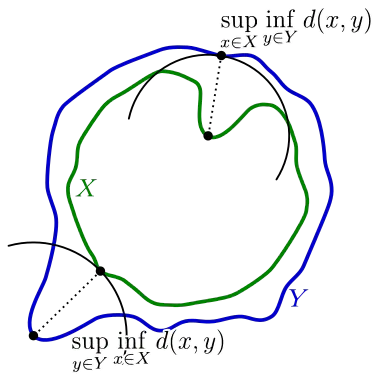
\includegraphics[width=.5\textwidth]{pics/Hausdorff distance.png}
	\caption{Hausdorff Distance}
	\label{fig: hausdorff distance}
\end{figure}

\paragraph{MRR}
Mean Reciprocal Rank, 常用来衡量搜索算法效果的指标, 目前被广泛用在允许返回多个结果的问题, 或者目前还比较难以解决的问题中 (由于如果只返回top 1的结果, 准确率或召回率会很差, 所以在技术不成熟的情况下, 先返回多个结果) . 在这类问题中, 系统会对每一个返回的结果给一个置信度 (打分) , 然后根据置信度排序, 将得分高的结果排在前面返回. 核心思想很简单: 返回的结果集的优劣, 跟第一个正确答案的位置有关, 第一个正确答案越靠前, 结果越好. 定义如下: 
$$
MRR = \frac{1}{|Q|} \sum_{i=1}^{|Q|} \frac{1}{rank_i}
$$
其中$Q$为查询集合, $rank_i$是第$i$个查询的结果集中正确结果的排名. 

\paragraph{AP}
Average Precision, 平均精确率. 对于二分类问题, 给定样本真实标签$\{y_1, ..., y_n\}$和模型预测的正样本置信度$\{c_1, ..., c_n\}$, 计算AP: 
\begin{enumerate}
	\item 按照置信度从大到小对样本进行排序, 令排序后的样本的置信度为$\{c_1, ..., c_n\}$
	\item 令 $i=1$, 重复执行: 
	\begin{enumerate}
		\item 以$c_i$为阈值, 得到预测的正负样本, 即前$i$行预测为正样本, 之后的均为负样本
		\item 计算当前阈值下的Recall和Precision
		\item $i += 1$
		\item 当$i > n$则结束循环
	\end{enumerate}
	\item 排序后的每个样本都对应一个(Recall, Precision)对, 即$\{(r_1, p_1), ..., (r_n, p_n)\}$
	\item 上一步得到的Recall列表$\{r_1, ..., r_n\}$中的元素$r_i$与$r_{i-1}$做差, 设$r_0 = 0$, 则可以得到$\{d_1, ..., d_n\}$, 其中$d_i = r_i - r_{i-1}$
	\item 求和: $AP = \sum_{i=1}^n d_i \cdot p_i$
\end{enumerate}
如Fig.\ref{fig:ap}所示, 该表是按照置信度排序后的样本, correct列表示该样本的真实标签, P、R列是按照上述方式计算出来的Recall和Precision. 
\begin{figure}[h]
	\centering
	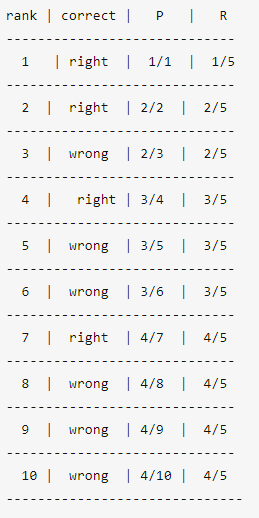
\includegraphics[width=.3\textwidth]{pics/AP.png}
	\caption{AP计算示例}
	\label{fig:ap}
\end{figure}

\paragraph{MAP}
Mean Average Precision, 是AP的均值. AP通常是针对单个类别而言的, 当有多个类别时, 分别计算每个类别的AP, 再进行算术平均. 

\tbc{red}{注意: }AP和MAP常用在目标检测和信息检索领域中. 
\begin{itemize}
	\item 目标检测领域中, 对于一个类别, 可能会检测出多个检测框, 每个检测框可以根据IoU来判断检测框的真实标签是1还是0 (针对一个类别的检测而言, \tbc{green}{因为目标检测中的Ground Truth也是一个边界框, 所以不需要和边界框完全一致才作为正样本, 只要IoU大于一定阈值即可}) , 每个检测框还对应一个置信度. 此时即可按照上述方式计算该类别的AP
	\item 在信息检索领域, 对于一个查询$q$, 通常希望模型能够给出top K个结果 (\tbc{red}{有序的}) . 若$q$真实的有序搜索结果列表为$\{d_1, ..., d_m\}$, 则可以对这K个结果的标签, 由于模型的输出已经是排好序的, 故可以直接计算AP. 对于多个查询, 则计算每个查询的AP后再取平均
\end{itemize}
总而言之, 根据某种方法判定样本的真实标签 (如目标检测中通过IoU判定、分类任务中给定的标签、搜索中给定的真实搜索列表等) , 再根据置信度进行排序 (如目标检测中的置信度、分类任务中输出的分数、搜索中直接给出的排序等) , 计算每个位置处的$(recall, precision)$, 按照上述方式即可算出AP. 


\paragraph{DCG、NDCG}
Discounted Cumulative Gain, 折扣累计增益. 在介绍DCG之前有必要先介绍一下CG, Cumulative Gain, 即累计增益. 这两个指标主要用于搜索领域. 对于模型返回的$p$个结果 (\tbc{red}{有序的}) , 每个位置处的结果与查询的相关性为$rel_i$, 则该结果的CG为: 
$$
CG_p = \sum_{i=1}^p rel_i
$$
很明显, CG没有考虑结果的先后顺序, 在搜索中, 结果的顺序是至关重要的, 因此产生了DCG: 同一个相关度, 排名越后则增益越小, 即与所处排名成反比. 
$$
DCG = \sum_{i=1}^p \frac{rel_i}{\log_2(i+1)}\qquad or\qquad \sum_{i+1}^p \frac{2^{rel_i} - 1}{\log_2(i+1)}
$$
通常, 不同的查询对应的结果列表是不一样长的 (\tbc{green}{不同长度的搜索结果对应的DCG值范围不一样, 无法直接比较, 例如长的结果列表DCG最大可为10, 短的最大可为5, 前者的DCG为4和后者的DCG为4并不代表二者的结果列表质量一样}) , 因此不能将DCG用于评价结果列表长度不同的查询效果, 因此需要对DCG进行归一化, 即NDCG (Normalized DCG, 归一化折扣累计增益) , 
$$
NDCG = \frac{DCG}{IDCG}
$$
其中IDCG为理想情况下的折扣累计增益, 表示真实的结果列表的DCG, 计算方式为取真实结果列表的前$p$个结果计算DCG, 即
$$
IDCG = \sum_{i=1}^p \frac{2^{rel_i} - 1}{\log_2(i+1)}
$$

\tbc{red}{注意: }MAP和NDCG都可以用于衡量搜索结果的质量, 但是MAP只支持两种相关性: \{相关, 不相关\}, NDCG可以支持多种相关性得分, 如1-5. 


\paragraph{GAUC}Group AUC, 是 AUC 的一个变体, 在推荐系统领域中更准确地衡量模型得性能. 以 CTR 估计任务为例, 数据集中包含了不同用户得正负样本, 模型给出每个样本属于正样本得一个概率值后计课计算一个 AUC. 但是很明显, AUC 将不同用户的正负样本混合起来了, 即期望任一个用户的正样本的概率大于任一个用户的负样本的概率, 但推荐中更关注的是对于一个用户, 模型对其正负样本的排序能力. 其定义为: 
$$
GAUC = \frac{\sum_{u_i} w_{u_i} \cdot AUC_{u_i}}{\sum_{u_i} w_{u_i}}
$$
其中 $w_{u_i}}$ 是 $u_i$ 的权重, 这个值可以是用户的样本的数量. 可以看出, GAUC 是定义在 AUC 上的, 即计算模型对每个用户的样本的排序能力. 其实可用通过这个指标发现模型对哪一类用户有较好的性能, 那是不是可以以此为基础进行多个模型的融合呢?

\subsection{常用数据增强手段}
增强之前, 先想一想: 真的需要增强数据吗 (通常来说是的) ?需要增加的多少数据?需要增加什么样的数据 (并不是什么样的数据都可以, 主要考虑应用场景中一般会出现的数据即可) ?
\paragraph{仿射变换}
仿射变换 (Affine Transformation) 是指在二维向量空间中进行一次线性变换(乘以一个矩阵)和一次平移(加上一个向量), 变换到另一个向量空间的过程. 
$$
\left[\begin{array}{l}
	u \\
	v \\
	1
\end{array}\right]=\left[\begin{array}{ccc}
	a_{1} & b_{1} & c_{1} \\
	a_{2} & b_{2} & c_{2} \\
	0 & 0 & 1
\end{array}\right]\left[\begin{array}{l}
	x \\
	y \\
	1
\end{array}\right]
$$

图解, 放射变换的种类也如Fig.\ref{fig:affine}所示: 
\begin{figure}[h]
	\centering
	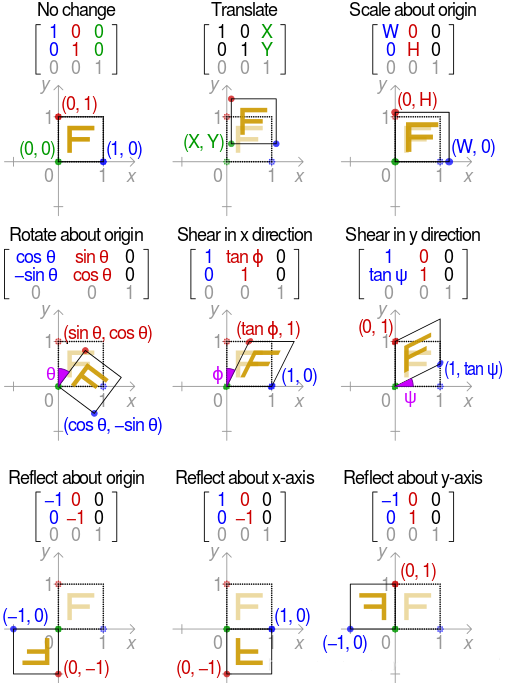
\includegraphics[width=.8\textwidth]{pics/affine.png}
	\label{fig:affine}
	\caption{仿射变换}
\end{figure}

\paragraph{弹性形变\cite{simard2003best}}
最早是从UNet中了解到弹性形变, 在细胞分割中, 弹性形变发挥了重要作用; 弹性形变也用在手写数字识别中. 可以发现, 在这两种任务中, 任务所涉及的对象并不是刚体, 简单的仿射变换并不能满足我们的需求. 弹性形变所针对的数据特点: 对象不是刚体, 可能在不同的场景下会有形变. 

弹性形变流程: 
\begin{itemize}
	\item 对图像imageA进行仿射变换, 得到imageB
	\item 对imageB图像中的每个像素点随机生成一个在x和y方向的位移, $\Delta \mathrm{x}$和$\Delta \mathrm{y}$. 其位移范围在(-1, 1)之间, 得到一个随机位移场(random displacement fields)
	\item 用服从高斯分布的$N(0, \delta)$对step2中生成的随机位移场进行卷积操作(和CNN中的卷积操作一样, 说白了就是滤波操作). 我们知道δ越大, 产生的图像越平滑. 下图是论文中的不同δ值对随机位移场的影响, 下图左上角为原图, 右上角为$\delta$较小的情况(可以发现, 位移方向非常随机), 左下角和右下角为较大的不同$\delta$值
	\item 用一个控制因子$\alpha$与随机位移场相乘, 用以控制其变形强度
	\item 将随机位移场施加到原图上, 具体是\textbf{怎么施加的呢}?首先, 生成一个和imageB大小一样的meshgrid网格meshB, 网格中的每个值就是像素的坐标, 比如说meshgrid网格大小为512x512, 则meshgrid中的值为(0, 0), (0, 1), ..., (511, 0), (511, 511), 然后将随机位移场和meshB网格相加, 这就模拟了imageB中的每个像素点在经过随机位移场的作用后, 被偏移的位置, meshB与随机位移场相加后的结果记做imageC
	\item 弹性变形最终输出的imageC中每个位置的灰度值大小, 组成一副变形图像, 现在imageC中每个像素点存储的是$(\mathrm{x}+\Delta \mathrm{x}, \mathrm{y}+\Delta \mathrm{y})$, 如下图中的$\mathrm{A}^{\prime}$, 那怎么转化成灰度值呢, 依据论文, 作者是根据imageB中的B位置的双线性插值灰度值作为$\mathrm{A}^{\prime}$点的像素灰度值大小 (如Fig.\ref{fig:elastic-deform}所示) , 最终将imageC输出得到变形图像
\end{itemize}
\begin{figure}[h]
	\centering
	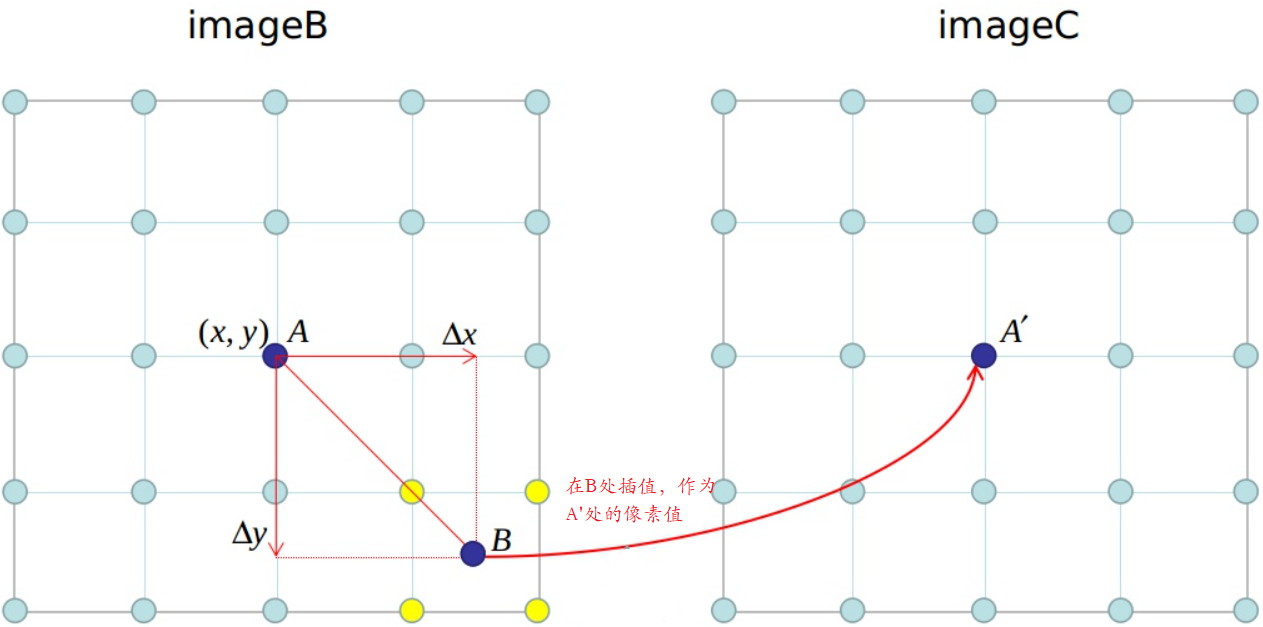
\includegraphics[width=.8\textwidth]{pics/elastic_deform.png}
	\label{fig:elastic-deform}
	\caption{弹性形变}
\end{figure}
参考: \href{https://zhuanlan.zhihu.com/p/342274228}{数据增强: 弹性变形(Elastic Distortion)}. 

\paragraph{增加噪声}
如椒盐噪声. 

\paragraph{GAN}


\subsection{类别不平衡问题}
指的是监督学习中, 不同类别的样本数目具有较大的差异 (样数据分布与均匀分布差异较大) . 
\paragraph{类别不均衡可能造成的问题}
\begin{itemize}
	\item 一些评价指标可能失效. 例如在癌症检测中, 可能$99\%$的样本都是0, 只有$1\%$的样本为1, 这个时候即使将所有样本预测为0也能有很好的acc, 但是漏检是很严重的!类别不平衡使得一些评价指标并不能反映模型真是的能力
	\item 
\end{itemize}

\paragraph{决解办法}
\subparagraph{数据角度}
中心思想就是直接改变数据分布. 
\begin{itemize}
	\item 获取更多数据, 使数据分布趋向于均衡
	\item 上采样. 通过一些方法, 使得占少数的类别 (minority类) 的样本数增加, 常用的方法: 
	\begin{itemize}
		\item 重复采样minority类, 使其样本数增加
		\item 合成的方法. 根据已有数据集生成新的样本, 如SMOTE方法及其变体
		\item 基于聚类. 分别对major和minority类进行聚类, 再通过过采样的方法使得major和majority中各个簇的数量相等, 例如原本major类聚类后样本数目比为1:2:3, minority类聚类后为1:2, 通过过采样的方法, 先使majority与minority样本数相等, 再使类内部各个簇的数目相等. 这样不仅可以解决类别间的不平衡, 还可以解决类内部的不平衡
	\end{itemize}
	\item 下采样. 通过一些方法把占多数的类别 (major类) 的样本数降低. 下采样的方法有很多
	\begin{itemize}
		\item 随机下采样, 从major类中随机保留一部分样本
		\item 基于临近样本, 来选择保留哪些major类样本
		\item 基于聚类, 对major类进行聚类, 使其具有N (minority类样本数) 个簇, 用这N个簇的中心作为major类采样后的样本
	\end{itemize}
\end{itemize}

\subparagraph{算法角度}
\begin{itemize}
	\item 选择对数据倾斜相对不敏感的算法, 如树模型等
	\item 在下采样时会损失一部分信息, 可以从major类中采样多个数据集来学习不同的模型, 即集成学习 (Ensemble集成算法) . 首先从多数类中独立随机抽取出若干子集, 将每个子集与少数类数据联合起来训练生成多个基分类器, 再加权组成新的分类器, 如加法模型、Adaboost、随机森林等
	\item 将任务转换成异常检测问题. 譬如有这样一个项目, 需要从高压线的航拍图片中, 将松动的螺丝/零件判断为待检测站点, 即负样本, 其他作为正样本, 这样来看, 数据倾斜是非常严重的, 而且在图像质量一般的情况下小物体检测的难度较大, 所以不如将其转换为无监督的异常检测算法, 不用过多的去考虑将数据转换为平衡问题来解决
\end{itemize}

\subparagraph{评价指标角度}
\begin{itemize}
	\item 混淆矩阵
	\item F-score
\end{itemize}

\subsection{特征选择的方法}
机器学习中, 面对成千上万的特征, 选择哪些进行保留是一个需要我们主动去抉择的问题. 既然是选择, 那肯定是要有一个明确的评判标准的. 

\subsubsection{过滤法}


\subsubsection{包装法}

\subsubsection{嵌入法}

\subsection{常用聚类算法}

\subsubsection{基于层次的聚类}
试图在不同层次上进行聚类, 从而形成树形的聚类结构. 数据集的划分可以自底向上也可以自底向下. 常见的有: Agglomerative 、Divisive、BIRCH、ROCK、Chameleon. 

\paragraph{优点}可解释性好 (如当需要创建一种分类法时) ; 还有些研究表明这些算法能产生高质量的聚类, 也会应用在上面说的先取 K 比较大的 K-means 后的合并阶段; 还有对于 K-means 不能解决的非球形族就可以解决了.  

\paragraph{缺点}时间复杂度比较高. 

\subsubsection{基于划分的聚类}
首先要确定簇的数量, 然后初始化簇的中心点, 再然后依据预先定好算法对数据点进行迭代重置 (即重置其所属的簇) , 直到最后到达“类内的点都足够近, 类间的点都足够远”的目标效果. 常见的有: K-means、K-means++、K-medoidsk-modes、k-medians、kernel k-means. 

\paragraph{特点}能够发现数据集中的球状簇, 因为通常是根据样本与中心的距离来划分的, 因此簇的表面通常是球面. 

\paragraph{优点}算法简单, 效率还可以. 

\paragraph{缺点}数据集较大时可能容易陷入局部最优 (\textcolor{red}{\textbf{为啥}}) ; 需要预先设定簇的数量 (看这些算法以 $k$ 打头就知道啦) ; 对异常值较敏感; 只适用于可计算相似性的样本空间. 
	
\subsubsection{基于密度的聚类}
定一个距离半径, 最少有多少个点, 然后把可以到达的点都连起来, 判断为同类. 常见的有: DBSCAN、OPTICS、DENCLUE. 

\paragraph{特点}能够对流形的数据进行聚类. 
	
\paragraph{优点}能够发现任意形状的簇, 对噪声不敏感. 

\paragraph{缺点}聚类的结果与参数有很大的关系; 当聚类的稀疏程度不同时, 相同的判定标准可能会破坏聚类的自然结构, 即较稀的聚类会被划分为多个类或密度较大且离得较近的类会被合并成一个聚类. 
	
\subsubsection{基于网格的聚类}
数据空间划分为网格单元, 将数据对象集映射到网格单元中, 并计算每个单元的密度. 根据预设的阈值判断每个网格单元是否为高密度单元, 密度足够大的网格单元形成簇. 常见的有: STING、WaveCluster、CLIQUE. 

\paragraph{优点}速度很快. 

\paragraph{缺点}参数敏感、无法处理不规则分布的数据、维数灾难等; 这种算法效率的提高是以聚类结果的精确性为代价的. 经常与基于密度的算法结合使用. 
	
\subsubsection{基于模型的聚类}
为每簇假定了一个模型, 寻找数据对给定模型的最佳拟合, 这一类方法主要是指基于概率模型的方法和基于神经网络模型的方法, 尤其以基于概率模型的方法居多. 这里的概率模型主要指概率生成模型 (generative Model) , 同一 "类" 的数据属于同一种概率分布, 即假设数据是根据潜在的概率分布生成的. 常见的有: GMM) 、SOM (Self Organized Maps) . 

\paragraph{优点}对”类“的划分不那么”坚硬“, 而是以概率形式表现, 每一类的特征也可以用参数来表达. 

\paragraph{缺点}执行效率不高, 特别是分布数量很多并且数据量很少的时候. 

主要参考: \href{https://blog.csdn.net/weixin_45440065/article/details/106358007}{聚类总结: 分类、优缺点、适用场景总结}、\href{https://blog.csdn.net/count_on_me/article/details/82193745}{聚类及聚类算法的分类}. 

\subsection{类别变量的编码方法}
\subsubsection{one-hot}
这个就很简单了, 将一个类别变量展开成一个向量, 向量的长度等于类别变量的基数. 经过独热编码后, 一个类别变量变成了一个向量, 很明显这增加了数据的维度, 而且编码后的数据是很稀疏的. 

\subsubsection{目标编码}
Target Encoder 是一种有监督的编码方式, 适用于分类和回归问题, 主要针对定类变量. 考虑分类问题. 假设在分类问题中, 目标 $y$  一共有 $C$ 个类别, 具体的一个类别用 $c$ 表示, 为了简化讨论, 当前考虑一个 $c$. 同时假设某一个定性特征 $f$ 中一共有 $K$ 个不同的类别, 具体的一个类别用 $k$ 表示. 针对一个目标 $c$, 目标编码将 $f$ 转化为一个后验概率 $P(y = c | f=k)$. 因此, 一个 $C$ 个类别的任务, 可以将 $f$ 转化成 $C-1$ 个特征, 每个特征针对一个目标进行编码. 即 $P(y=c_i | f=k), i=1, ..., C-1$. 

但是这样的做法有一个问题, 经过目标编码后的特征与目标有很强的相关性, 容易发生过拟合. 可以对目标编码进行平滑: 
$$
P = (1-\lambda) \cdot P(y = c) + \lambda \cdot P(y=c | f=k)
$$
一个特征类别在训练集内出现的次数越多, 其后验概率的可信度越高, 所以其权重也应该适当增大, 即此时 $\lambda$ 应该越大; 相反, 如果当一个特征类别在训练集内出现的次数较少的时候, 其后验概率的可信度较低, 所以我们应该让正则项更强一些, 即应该减小 $\lambda$. 那 $\lambda$ 应该如何取值呢?$\lambda$ 应该是一个关于某个特征类别在训练集中出现的次数 $n$ 的函数, 输出是对于这个特征类别的先验概率的权重的函数. 一种常用的计算方式: 
$$
\lambda (n) = \frac{1}{1+e^{-\frac{n-\beta}{\alpha}}}
$$
其中引入了两个参数 $\alpha, \beta$. 很明显, 当 $n > \beta$ 时 $\lambda > 0.5$, 即后验概率占比更大, 反之亦然. $\alpha$ 用于控制拐点处的斜率, 越小, 斜率越大.  

\subsubsection{贝叶斯目标编码}

\subsubsection{留一编码}

\subsubsection{证据权重}

\subsubsection{非线性 PCA}

\subsubsection{Embedding}

\subsection{为什么分类问题使用交叉熵而不使用 MSE?}
MSE 作为损失函数是非凸的, 不容易求解, 容易得到局部最优解; 而交叉熵损失函数是凸函数. 

MSE 求导后, 梯度与 sigmoid 的导数有关, 容易落在 sigmoid 的平坦区, 导致梯度很小, 引发梯度消失问题; 交叉熵求导后梯度为残差, 误差越大更新越快, 误差越小更新越慢. 

交叉熵衡量的是预测的分布与真实分布的距离, 更符合分类问题的预测目标.

\subsection{为什么要将连续特征离散化后输入到线性模型中?}
连续值经常离散化或者分离成 “箱子” 进行分析, 为什么要做数据分桶呢?
\begin{itemize}
	\item 离散后稀疏向量内积乘法运算速度更快, 计算结果也方便存储, 容易扩展; 
	
	\item 离散后的特征对异常值更具鲁棒性, 如 age>30 为 1 否则为 0, 对于年龄为 200 的也不会对模型造成很大的干扰; 
	
	\item LR 属于广义线性模型, 表达能力有限, 经过离散化后, 每个变量有单独的权重, 这相当于引入了非线性, 能够提升模型的表达能力, 加大拟合; 
	
	\item 离散后特征可以进行特征交叉, 提升表达能力, 由 M+N 个变量编程 M*N 个变量, 进一步引入非线形, 提升了表达能力; 
	
	\item 特征离散后模型更稳定, 如用户年龄区间, 不会因为用户年龄长了一岁就变化; 
	
	\item 特征离散化以后, 起到了简化了逻辑回归模型的作用, 降低了模型过拟合的风险; 
\end{itemize}


\subsection{分类模型与排序模型的异同分析}
\textbf{注意}: 这一节内容主要参考\href{https://zhuanlan.zhihu.com/p/502638808?utm_source=wechat_session&utm_medium=social&utm_oi=797192809567354880&utm_campaign=shareopn}{这里}.

在初入推荐系统这个坑时就思考过推荐和搜索的差异与异同, 那时我肯定想不到现在就在做搜索相关的实习. 缘分呐, 搜索!

不管在推荐还是搜索中, 都可以归结为 \textit{Learning To Rank}(LTR). LTR 通常由三种形式: Point-Wise, Pair-Wise 和 List-Wise. 推荐中, 排序的依据通常是 Point-Wise 形式的, 很多情况下就是 CTR, 这个问题可以看作是一个二分类的问题. 在搜索中, 就我目前了解到的情况来看, 更多的是 Pair-Wise 的 (仅就我目前了解到的情况).

\subsubsection{建模角度}
就二分类而言, 大多数模型最后输出的概率值都是通过 \textit{sigmoid} 得到的, 这就隐含了一个假设, 即假设样本为正样本的概率服从二项分布. 以逻辑回归为例, 在进入 \textit{sigmoid} 之前, 模型的值表示的是对数几率, 即 LR 线性部分预测的是对数几率. 真实的 CTR 模型也是类似的含义.

排序模型, 可以采用 LTR 的三种形式, 但使用较多的是 Pair-Wise, 这里就以这个为例吧. 在 Pair-Wise 中, 对于两个文档, 预测的是偏序关系是否成立:
$$
P_{i j} = P_{i} > P_{j}
$$
$P_{ij}$ 表示的是 $i$ 比 $j$ 排名更前的概率. 其实 $P_{ij}$ 也可以看作是一个分类变量, 但此时我们的样本是 $(i, j, P_{ij})$. 因此, 类比于二分类中的交叉熵损失:
$$
PairLoss = \sum_{(i, j) \in \{pairs\}} -P^\prime_{ij} \log P_{ij} - (1 - P^\prime_{ij}) \log (1 - P_{ij})
$$

综合对比来看, 推荐中的 Point-Wise 和搜索中的 Pair-Wise, 都可以看作是一个二分类变量, 差别在于二者的样本上. 推荐中估计的是单个样本的点击率, 搜索中估计的样本对的偏序关系是否成立. \textbf{\textcolor{red}{这二者来排序有啥不同呢?}} 在分类模型中, 要对两个样本都有准确的预估才能保持正确的派内需关系, 其要求更高; 而 Pair-Wise 可以看作分类模型的一个简化版本, 只要求偏序关系正确, 不要求对单个样本的预估绝对准确.

\subsubsection{事件之间的相互独立性假设} 
其实从二者的建模角度来看就可以看出, 分类模型假设各个样本之间是相互独立的 --- 独立同分布; Pair-Wise 则建立在同组 (同一个 query) 样本可以比较的基础上. 

\subsubsection{参数更新方式}
假设 $f$ 是要学习的模型, 在分类中代表分类模型, Pair-Wise 中代表对每个文档进行打分的模型 (类似于双塔). 则损失函数对参数的导数为:
$$
\frac{\partial L}{\partial w}=\frac{\partial L}{\partial f} \frac{\partial f}{\partial w}
$$

则 Point-Wise 的参数更新为:
$$
\mathrm{w}_{\mathrm{i}}^{\mathrm{t}+1}=w_{i}^{t}+\eta \frac{\partial L}{\partial f} \frac{\partial \mathrm{f}}{\partial w_{i}^{t}} \mathrm{x}_{\mathrm{i}}
$$

Pair-Wise 的参数更新为:
$$
\mathrm{w}_{\mathrm{i}}^{\mathrm{t}+1}=w_{i}^{t}+\eta \frac{\partial L}{\partial\left(f^{+}-f^{-}\right)} \frac{\partial\left(f^{+}-f^{-}\right)}{\partial w_{i}^{t}}\left(\mathrm{x}_{\mathrm{i}}^{+}-\mathrm{x}_{\mathrm{i}}^{-}\right)
$$
其中 $f^+, f^-$ 分别表示排名在前, 在后的样本的打分. 可见, 二者的偏序关系越显著, 参数更新的幅度越大.

\subsection{WOE, IV}
WOE, Weight of Evidence, 常用在风险评估、授信评分卡等领域. 

WOE是对原始自变量的\textbf{一种编码形式}, 要对一个变量进行 WOE 编码, 需要首先把这个变量进行离散化. 以二分类为例, 当拿到了一个离散变量, 对其进行 WOE 编码地过程: 按照变量的取值对数据集进行划分, 统计每个取值里正负样本的数量及在总的正负样本里的占比. 比如说, 变量 A 的取值 $a_1$ 中, 正负样本量分别是 $p, n$, 在总的正负样本量分别为 $P, N$, 则 A 变量的 $a_i$ 的 WOE 编码为 $ln \frac{p / P}{n / N}$. 通过 WOE 的计算公式也可以看出, 通常会在计算时加入平滑项避免 $p, n$ 为 0  的情况.

WOE 编码的好处:
\begin{itemize}
	\item WOE 是一种比较好的把自变量转化为与\textbf{对数几率}线性相关的有效形式;
	
	\item 所有自变量被 WOE 编码标准化后, 求解得到的系数值取值都在同一范围, 可以直接比较不同自变量对 odds 的影响;
	
	\item WOE 能反映自变量的贡献情况. 自变量内部 WOE 值的变异 (波动) 情况, 结合模型拟合出的系数, 构造出各个自变量的贡献率及相对重要性. 一般地, 系数越大, WOE 的方差越大, 则自变量的贡献率越大;
\end{itemize}

IV, Information value, 可通过 WOE 加权求和得到, 衡量自变量对因变量的预测能力, 可用于筛选变量. IV 是在 WOE 的基础上计算得到的. 还是刚刚的例子, 变量 A 的取值 $a_i$ 的 IV 计算为: $(\frac{p}{P} - \frac{n}{N}) \cdot WOE_{a_i}$. 

那么如何通过 IV 进行变量筛选呢? 对于一个 $n$ 个取值的离散变量, 其 IV 值计算方式为 $\sum_i^n IV_{a_i}$. IV 值越大则变量的预测能力越强, 一般而言大于 0.2 则有较强的预测能力. 

关于 IV 的几个特点:
\begin{itemize}
	\item 分箱的数量对 IV 取值有影响, 分箱越多则 IV 会偏大;
	
	\item 使用 IV 进行变量选择时, 通常是针对 LR 模型而言, 对于其他的而分类模型不太使用. 因为 IV 的计算是建立在 WOE 上, 而 WOE 其实计算的几率;
\end{itemize}

参考资料: \href{https://zhuanlan.zhihu.com/p/74165987}{WOE与IV值浅谈}.

\subsection{特征交叉}
在做机器学习或者深度学习中, 特征工程都是必不可少的一个叫环节, 这其中就包含着构造特征, 根据业务场景构造交叉特征. 做特征交叉好像成了一种常规操作, 但是特征交叉为什么有效呢, 该怎么做呢?

\paragraph{为什么特征交叉有效}
通过特征交叉, 模型可以学习到特征间的非线性关系. 早期使用的模型大多是线性模型. 线性模型具有一些优点, 如计算复杂度相对较低, 解释下更好, 容易部署上线等. 但是线性模型难以发现变量之间的非线性关系. 因此有一些方法致力于在线性模型中引入非线性, 如 SVM 中的核函数, 手动构造交叉特征, FM, FFM, GBDT-LR 等. 首先一点需要确定的是, 交叉特征肯定是有效的, 如 \textit{性别}=\textbf{女} AND \textit{年龄}=\textit{青年}, 显然该特征对购物点击来说无疑是贡献很大的. \textbf{如果不加这样一个特征, \textit{性别}和\textit{年龄}这两个特征的线性组合能达到同样的效果吗?} 有一个简单的例子: 输入为 $x_1, x_2$ 的 XOR 问题. 这是线性不可分的, 但是如果引入交叉特征 $x_1*x_2$, 则问题就变成线性可分的了. 

但是如果模型本身就是非线性的, 如树模型, 深度模型, 还有必要做特征交叉吗? 从现有的情况来看, 大量的泛 Wide\&Deep 模型中依然要做特征交叉, DNN 部分不仅要做, 而且还要通过 Wide 部分做交叉特征. 可见, 非线性模型中也是有必要做特征交叉的. 这其实又引出来一个问题, DNN 做特征交叉的缺陷在哪?

\paragraph{怎么做特征交叉}
根据问题场景, 手动构造一些交叉特征这当然是必不可少的. 


\subsection{bagging 和 boosting}
集成学习的不同方式. 

boosting 是一种串行学习基学习器的集成方法, 每次训练一个基学习器, 根据基学习器的表现对训练样本的分布进行调整, 再进行后续的学习. bagging 则是并行地学习多个基学习器, 一般每个基学习器是在数据集的子集上训练的 (包括行采样和列采样). 

\textbf{二者的区别}:
\begin{itemize}
	\item 一个是串行的, 一个是并行的;
	
	\item 训练集不同. boosting 中会调整样本的权重, 而 bagging 会对原数据集进行采样;
	
	\item 结合方式不一样. boosting 一般是加权求和, bagging 中多是投票的方式;
	
	\item 方差-偏差. boostign 主要关注降低偏差, bagging 主要关注降低方差. boosting 通过赋予预测错误的样本更高的权重, 来逐步降低预测的偏差. bagging 通过采样的方法为不同基学习器生成不用的训练集, 虽然各个子集之间有一定相关性, 但在一定程度上也能降低方差.
\end{itemize}

\subsection{线上线下不一致的原因}
离线训练好的模型上线后, 可能会出现线上线下的结果不一致的情况, 比如离线有提升而线上反而下降了. 可能的原因:
\begin{itemize}
	\item 线上线下数据处理方式不一致;
	
	\item 特征更新延迟;
	
	\item 离线训练过程中出现问题, 比如说数据划分的不合理, 数据穿越, 过拟合等;
	
	\item 离线指标不合理. 离线指标并不等价线上观测的指标;
	
	\item 线上观测不全面. 可能模型的效果确实提升了, 但是线上观测的样本不足或者数据分布有问题;
\end{itemize}